\documentclass[a4paper]{article}
\usepackage{lipsum}
\usepackage{url}
\usepackage{graphicx}
\usepackage[margin=2cm]{geometry}
\graphicspath{ {images/} }

%Custom Commands
\newcommand{\Pokemon}{Pok\'{e}mon}


\begin{document}

%Title Information
\title{
    Project Proposal
    \\ \large{G53IDS}
    \\ \large{Project Title: Applying Evolutionary Algorithms to \Pokemon{} Team Building}\vspace{-3ex}}
\author{4262648 Benjamin Charlton (psybc3)}
\date{\vspace{-2ex}11\textsuperscript{th} October 2017}
\maketitle

\section{Background and Motivation}
Video games are an ever growing field of interest for many people. Like many games people play competitively against each other and in some cases their are tournaments on an international scale with whole teams set up to win the large prize pools\cite{eSportsPrize}\cite{teamEarnings}. This field has become to be known as eSports.\\
Game playing is an obvious application of AI techniques as you can objectively score wins and losses. Initially this has been seen with traditional board games like Chess\cite{deepBlue} and Go\cite{alphaGo}. During The International 2017 for DotA 2 this all changed as the worlds of AI and eSports came together in a 1v1 show match\cite{openAI}. Elon Musk, backer of this initiative, said that this is `Vastly more complex than traditional board games like chess \& Go'\cite{openAI}.Typically in these set ups their is no decisions to be made prior to the game itself, in fact to limit the DotA 2 AI they limited it to a preselected character to play with.\\
Many strategy games have decision making before the game is played. Collectable Card Games (CCGs) have the choice of which cards to put in your limited deck or in \Pokemon{} you have to choose which members of your team to use and how you have trained them. This element of the games is refereed to as deck/team building as the player has to build up what they bring to the game from an empty deck or team. Some players are very good at playing the game but not very good at choosing which deck/team to bring resulting in a practice called `netdecking', being called so as the player will take someone else's deck/team from the internet instead of coming up with their own.\\
\Pokemon{} has a tricky team building process that is rather hard for new players to comprehend. In the build up to the annual \Pokemon{} World Championships, many players will go through the tedious process of team building to make sure they have the right strategies and counters in place to bring to the matches ahead\cite{worldsOverview}. This requires expert knowledge such as type match ups and speed tiers along side several rules of thumb. Once a general strategy is in place the players must perform several calculations to optimise the statistics of their team, optimising offensive stats to faint certain threats or optimising defensive stats to allow the team to survive after certain moves are used against them.\\
An attempt at automating the deck building process via evolutionary algorithms have been made in Hearthstone, a popular CCG\cite{hearthstoneAI}. The results where comparable of a well designed human deck which a talent player could then go and take to win tournaments. Another evolutionary algorithm was created to optimise build orders in StarCraft 2, a real time strategy game. The solution that the AI came up with was quicker than the best known strategy at the time and went on to be used in competitive play\cite{starcraftEA}\\
\Pokemon{} team building is a similar problem to the other deck building problems stated. These where solved to an respectable standard by evolutionary algorithms and as such it seems worthwhile to try and apply this method to the problem.

\section{Aims and Objectives}
This project aims to implement a evolutionary algorithm that will team build for \Pokemon{}. The output of such will be a team of \Pokemon{}, including all of the vital statistics and moves. This would be dependant of the format. These results will be then compared to human designed solutions to conclude if the evolutionary algorithm is any better than a expert.\\
\\The objectives of this project are:
\begin{enumerate}
    \item Research evolutionary algorithm methods used to approach similar problems. Looking in detail about issues such as representation, evaluation and validity of the chromosomes. This information will be used to help direct how best to approach the problem and design the system.
    \item Design an effective and efficient way to model and represent the problem in the evolutionary algorithm while still maintaining relevant data to the problem. This will also be used to form the output so will need to be readily be able to translate into a readable format for the user to understand.
    \item Develop a Genetic and Memetic algorithm to tackle the problem from scratch, including conventional and unique methods for the various stages in the algorithms. Making sure that all of the elements of the code base are created in a fashion that allows for reusability and adaptation. For example both the Genetic and Memetic algorithm should share the methods like objective evaluation and selection.
    \item Compare and analyse the results of each evolutionary algorithm (with a variety of settings) with each other and human designed solutions. Solutions for comparison will come from readily available teams from top players and analysis will be taken by evaluating the solutions. If solutions are viable enough they can be input into the game and used in some real world settings such as battling with other players, rather than being graded by a score.
\end{enumerate}

\section{Work Plan}
To help outline the project flow and I have created a gantt chart (found in the appendix) and the following descriptions of each portion.

%Explanations of all of the Points on the work plan
\begin{description}
\item [\large{Documentation}]
\item [Project Proposal] Write the project proposal and ethics form for approval of supervisor, due 13\textsuperscript{th} October.
\item [Revised Project Proposal] Any revisions to the project proposal that need to be made after supervisor feedback, due 23\textsuperscript{rd} October
\item [Interim Report] Write the interim report summarising the work so far, due 8\textsuperscript{th} December.
\item [Structure Sections] Decide and begin to structure the sections and the arguments within them for the final dissertation.
\item [Dissertation] Write the final dissertation, due 24\textsuperscript{th} April.

\item [\large{Research}]
\item [Evolutionary Algorithms] Research into the various Evolutionary Algorithms, like Genetic Algorithms, Memetic Algorithms \& Multimeme Memetic Algorithms.
\item [Review languages for EAs] Primarily seeing if python has suitable features required to make the development of evolutionary algorithms easier or whether Java would be better suited.
\item [Representation] Look into various representation methods that could be applied to the problem.
\item [Advanced EA Methods] Research the variety of more advanced methods for elements in evolutionary algorithms like selection and cross over.
\item [Memetic Algorithms] Study how memetic algorithms differ from genetic algorithms and why they are advantageous.

\item [\large{Development}]
\item [Create GA Structure] Set up the basic main loop and the relevant interfaces.
\item [Representation] Code the structure that the model will be represented by to be used as chromosomes in the Evolutionary Algorithm.
\item [Data import] Build methods to import the data that is needed at various points in the running of the algorithm.
\item [Validation Method] Build a method that will check that a chromosome is valid, for use after other methods so that invalid solutions aren't created.
\item [Basic Methods for GA] Create trivial methods for each stage of the Genetic Algorithm to allow for test runs.
\item [Bug Fixing 1] A period of time to allow for bug fixing and general code clean up to happen on the initial part of the project.
\item [Advanced Methods for GA] Create more advanced methods for the GA that may perform better.
\item [Memetic Algorithms] Code the structure of the memetic algorithm main loop and allow it to access the various methods created for the genetic algorithm. This could include creating more methods if research suggests that would be helpful.
\item [Bug Fixing 2] Another period for bug fixing, during this period all of the features should be locked in place.

\item [\large{Miscellaneous}]
\item [Install Software] Install and configure the relevant software and libraries that are required for the project.
\item [Run Basic Methods] Run the basic methods created with varying parameters to see some initial results

\item [\large{Other Commitments}]
\item [Welcome Week] First week of the year, time set aside to allow for settling in as well as running various welcome events.
\item [Christmas Holiday] Time off after Autumn term, Although not completely set aside allows for some time to relax.
\item [Autumn Exams] Potentially could have exams for the entire 2 weeks so is set aside to allow for revision and the exams themselves.
\item [Easter Holiday] Time off after Spring term, As no teaching is happening will give more time to concentrate on coursework and dissertation.
\end{description}

\section{Appendix}
%Bibliography
\bibliography{ProjectProposal}
\bibliographystyle{plain}

%Work Plan
\clearpage
\begin{center}
    \Large{Work Plan}\\
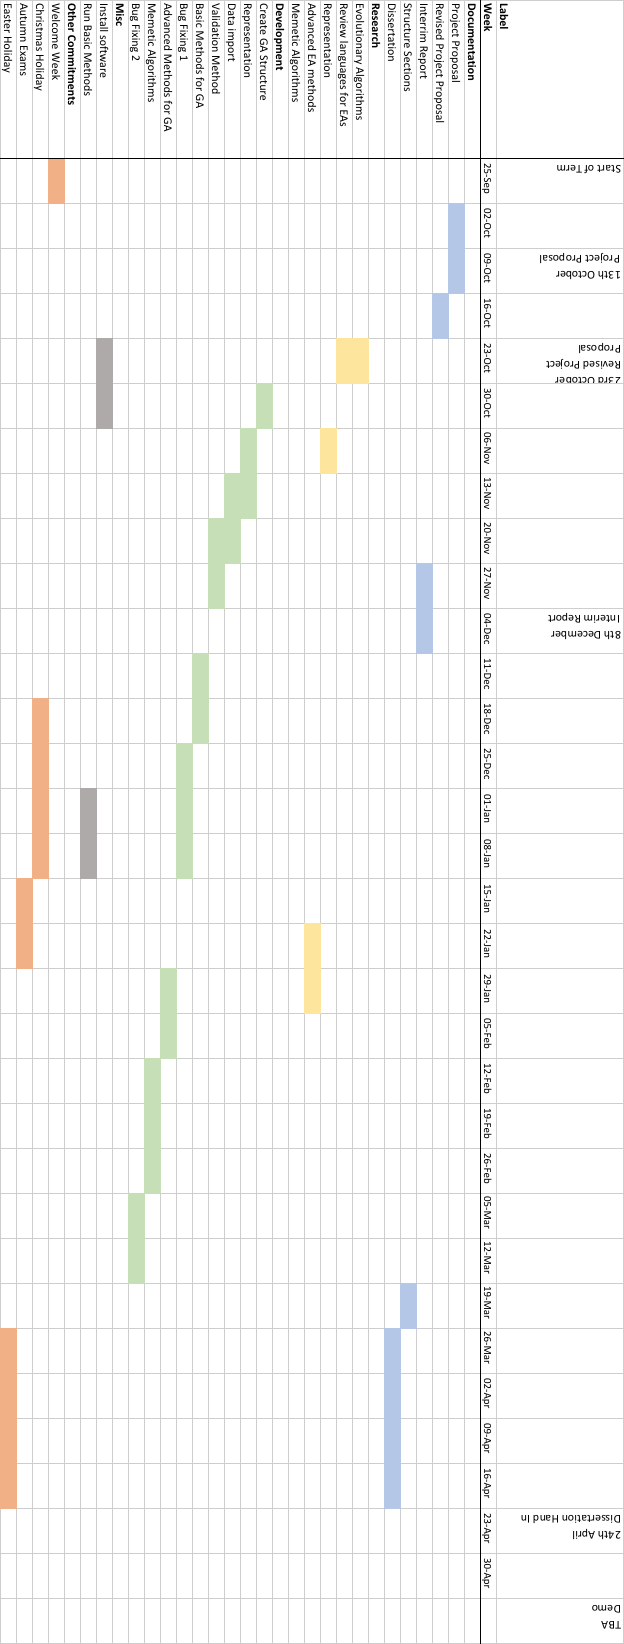
\includegraphics[height=24.8cm]{workPlan.png}
\end{center}


\end{document}
